\chapter{Introdução} \label{intro}

\lstset{language=Java}
\lstinputlisting[caption=Exemplo de como inserir um arquivo com c妖igo fonte,
label=code:Parser.java] {code/Parser.java}

\begin{figure}
\centering
\caption{Exemplo de como inserir uma figura}\label{fig:eela}
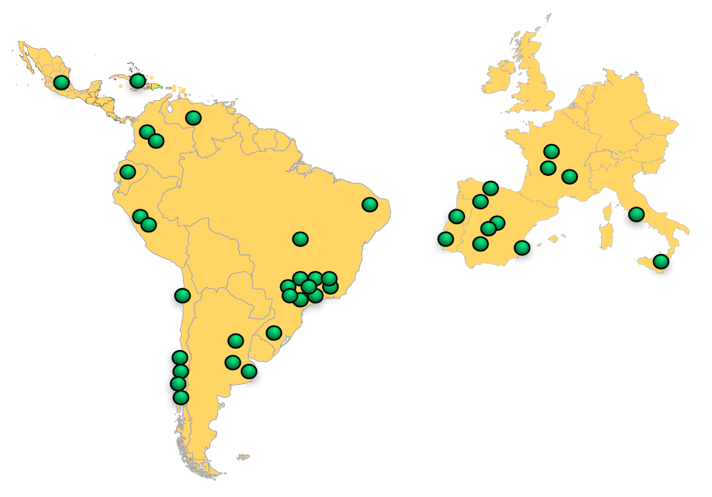
\includegraphics[width=0.7\textwidth]{images/eela.png}
\end{figure}


\begin{table}
\centering
\caption{Exemplo de como inserir uma tabela}\label{tab:exp-app}
\begin{tabular}{ | l | c | c | c |}\hline
 				   & Falha App. & Falha SE & Falha CE\\\hline
Resultado Esperado & 1.052       & 0        & 0       \\\hline 
Resultado Obtido   & 1.052       & 0        & 0       \\\hline 
Resultado Real  & 991        & 37       & 24      \\\hline 
\end{tabular}
\end{table}


\section{Motivação}\label{sec:motiva}

Aqui vai um exemplo de como citar uma refer刃cia contida no arquivo main.bib \cite{nakada2007job}.

\section{Objetivos}

\subsection{Objetivo Geral}

\subsection{Objetivos Especificos}

\section{Metodologia}

\section{Publicações Relacionadas}

\section{Estrutura da Dissertação}